\chapter{Related work}

\section{TODO2 Motivation} 
Although artificial intelligence has been a household name since the 1950s \cite{Rosenblatt58theperceptron:}, it has been experiencing a new boom for some years now, the end of which is not yet in sight.
The main reason for the ongoing high interest is the continuously increasing number of cases where machine learning (ml) outperforms man many times over, even with relatively low cost.
This could be achieved by the ever-increasing computing power, which together with the continuing achievements in research, all of a sudden, made things possible that were considered unsolvable some decades ago.
An example of this event is deep blue, a chess computer which in 1996 was able to beat the then world champion in chess, Garry Kasparov. What was a revolution at that time is rather unimpressive today, because everyone who owns a mobile phone with a chess app has a much more powerful tool in his pocket. [todo source, ich mach hier kein schach?]

Today, not only are far more complex problems being solved , ki is also becoming more and more prevalent in everyday life. [genes, alpha go][todo, speech recognition, word spelling, other assists, smart home, recommendations].

\section{Machine learning with neural networks}


\subsection{Supervised learning}

Supervised learning [todo image] is the task of learning a function that, for any given data, maps inputs to outputs only by training on samples of known data. This is mostly done by using neural networks which derive a mapping from the inputs to outputs. An example is labeling animals on image inputs correctly or recognizing handwritten letters.  [todo cite?]  

\subsection{Reinforcement learning}
Reinforcement learning [todo image] features an agent which has the task of learning the optimal behaviour in an environment without any default knowledge. To do so, the agent receives a reward for actions it performed as well as the state of the environment that it is currently in. In order to choose the best action, the agent has to learn a policy for all possible states. To improve the policy, the agent both has to exploit the experience that was made in the past, but also has to explore new possible solutions. This is called the exploration-exploitation tradeoff. [todo cite]

The problem is similar to supervised learning as a mapping from inputs to outputs has to be learned with the main difference being that no ``right'' decisions are known.
Well known examples are bots playing computer games like pong, doom or chess. [todo cite][todo images] For a long time, reinforcement learning was limited to rather simple, discrete problems. When state spaces are very large, for example in chess or in games with multi-dimensional continuous state spaces like 3d games have to be approximated. An option to do so is tiling [todo cite], but the major breakthroughs were achieved by using neural networks aswell. In reinforcement learning, they can be used to perform exactly this mapping.

\subsection{Neural networks}

\cite{Rosenblatt58theperceptron:} 
In order to find out whether and how one can resolve the logic within a neural network, we have to take a closer look at the functionalities.

Artificial neural networks are computing systems inspired by the biological brain. Such systems ``learn'' to perform tasks by considering examples, generally without being programmed with task-specific rules. The brain is made up of neurons which can activate each other to lead to a decision.

An artificial neural network is modeled with artificial neurons that are strung together in form of layers. The layers are connected in series between the neurons can communicate with each other. To calculate its own activation, a neuron receives signals from neurons in the proceeding layer. Every incoming signal gets multiplied with a specific weight which then is summed up and put into an activation function. The resulting activation is then sent to a set of neurons in the next layer. If the resulting output is correct, the weights can stay the same. If it is wrong though, the error is fed back through all layers with an algorithm called backpropagation where the weights are adjusted to support making the right decision next time.

\input{tikz/neural_networks/neural_network_layers}

\begin{figure}
    \centering
    \input{tikz/neural_networks/artificial_neuron}
    \caption{Artificial neuron with three input values}
    \label{tikz artificial neuron}
\end{figure}

Popular activation functions are the sigmoid function:
${sig}(t) = \frac{1}{1 + e^{-t}}$
aswell as the rectified linear unit function (ReLu):
$f(x)=\max(0,x)$

\begin{figure}
    \centering
    %\hrulefill
    %\fbox{
        \begin{minipage}[t]{0.40\textwidth}
        \input{tikz/neural_networks/graph_relu}
        \end{minipage}
        %}
    \hspace{5mm}
    %\fbox{
        \begin{minipage}[t]{0.40\textwidth}
        \documentclass{standalone} %[varwidth=\maxdimen,convert,border=5pt]
\usepackage{pgfplots}
\usepackage{tikz}
\usepackage{amsmath}
\begin{document}

\centering
\resizebox{\columnwidth}{!}{
    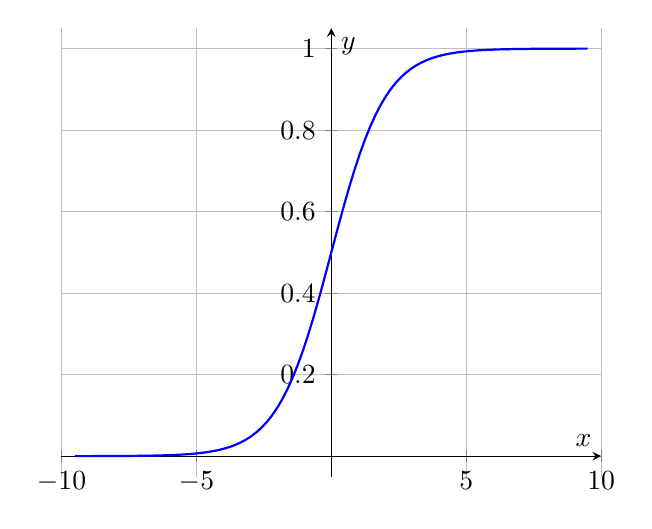
\begin{tikzpicture}
    \begin{axis}[
        grid=major,
        axis lines=middle,
        xmax=10,
        xmin=-10,
        ymin=-0.05,
        ymax=1.05,
        xlabel={$x$},
        ylabel={$y$}
    ]
    \addplot [domain=-9.5:9.5, samples=100, thick, blue] {1/(1+exp(-x)};
    \end{axis}
    \end{tikzpicture}
}

\end{document}
        \end{minipage}
    %}
\end{figure}


Artificial neural networks are computer systems that are strongly oriented towards the biological brain. An input vector is received by neurons, which in turn can activate other neurons. At the end of this process there are some neurons that can control an action.
In royal neural networks this principle is abstracted in layers of neurons. An input layer receives all important information and an output layer evaluates all possible actions - the best one is then taken. Between the two layers there can be any number of hidden layers. Their task is to divide the problem between the input layer and the output layer and to identify subproblems. The training process will be started with a random parameterization and the decisions will be very bad at the beginning. If a wrong decision is made, the neurons from output to input adjust their values so that the next time the right decision is made.

A neuron is modeled as follows (see Neuron). For a group of neurons from the previous layer (often all neurons) the signals are received and weighted. Together with a bias, which is added by the neuron itself, a sum is formed. To prevent unnaturally large values in neurons, the sum is added to an activation function that calculates the final activation of the neuron. Common activation functions include ReLu and Sigmoid. The result is then passed on to the neurons of the next layer.

The complexity of such a network depends on the number of layers, the number of nodes per layer and the type of interconnection between layers.
A possible network to solve Mountain Car could be for example an input layer with two neurons and an output layer with three neurons, as well as three hidden layers with 24, 48 and 24 layers each. Full connectivity between the layers is not unusual, resulting in the following number of connections:

 $2 \cdot {input} \cdot 24 \cdot 48 \cdot 24 \cdot 3 {output} = 165888$
 [todo formeln einfügen?]
the system thus consists of n $165888$ variables.

There is one thing that is decisive for the explainability: no matter at what point in time the network is viewed, it always has the same complexity. The only way to get better is to adjust the values within the given complexity.
connections (excluding $w_0$) and 101 neurons. [https://towardsdatascience.com/reinforcement-learning-w-keras-openai-dqns-1eed3a5338c] 

Over the years, many architectures of neural networks have been developed, which can often solve a specific problem very well. Worth mentioning are [todo, such as: convolutional neural networks, lstm, autoencoder, numerous activation functions, mcts, dqn double dqn, rainbow, ... Soll ich ein paar erwähnen?]. \cite{AIINDEX2019} 

[todo, wie genau Seitenzahl zitieren bei häufigerer Zitierung?]

\section{ML failure examples}

The continuing trend in the field of artificial intelligence also harbours some inconvenience.

In 2018, the Tesla autopilot caused a fatal accident because it mistook a truck standing crossways for a road sign. In 2015, one company caused a stir by claiming to have played a major role in the presidential election in America and the Brexit decision in Great Britain by means of data mining. Elon Musk and Stephen Hawking have both explicitly warned about the risks of artificial intelligence.
Apart from these horror scenarios, there are other reasons why it is not easy to dispense with the explanations.

\begin{itemize}
    \item How can false decisions be solved? Debugging and correcting false decisions by hand is almost not possible. How do I find out why a wrong decision was made? How can I change the behaviour without making mistakes in other places?
    \item How can you guarantee behaviour?
    \item How can you integrate small changes to the requirements of a neural network without new training processes?
    \item How can I apply this approach in a delicate environment?
    \item How to convince another person of my solution?
    \item How to justify in court a wrong decision of a machine?
    \item Even small changes in demand lead to a new training process
    \item Non-experts do not feel confident using the solution [todo zitat]. Rumours of machines learning to be evil [TODO rewrite] are widespread [TODO Zitat].
\end{itemize}

\subsection{Explaining how neural networks make decision}

Neural networks are insanely complex at all times. The attempt to gain information by analysing the values of neurons is therefore doomed to failure from the outset. Nevertheless, there are ways to extract information from the network. One possibility, is to look at the decisions and try to identify a structure behind them. It is also possible to look at parts of the neural network in isolation in order to deduce their function.

\subsection{Trusting a neural network}


Machine learning approaches can not be verified, the reliability can not be ``guaranteed''. Even more, they knowingly perform very poorly during the start of the training process. The trust into the reliability solely comes from its outstanding performance. A neural network will only be accepted as solution when the fail rate is so low that it is statistically insignificant. 

\subsection{Sensitive environments}

Companies that work with sensitive environments are particularly interested in preserving the explainability. We are certainly still a long way from having a nuclear power plant controlled by a neural network, but there are many areas where a controller makes decisions for a system where, in addition to many very good decisions, one single, wrong decision can lead to very great damage, for example to a gas turbine.
environments like these make it impossible for an agent to explore, so RL cannot be used or only with great restrictions.





\section{What is considered explainable?}

There are neural networks from which humans can extract information extremely easily: Our own brain. It is not only the most complex structure in the universe, it is also more energy-efficient than all artificial versions and, moreover, it already has a lot of instinct and life experience. physics applies everywhere to the same extent, which is why solutions found in certain areas can often be transferred to others in a similar form. [todo cite, idea] developers and experts have the wonderful ability to extract this information so efficiently that they can formulate a heuristic as a program after a short training period, often without any training at all.

Programs are probably the simplest way to describe a complex function.

Good coding style is a virtue even among experienced developers. In order to be able to understand programs written by computers as far as possible, special quality criteria apply. For our approach we have introduced some original features to achieve this.
